%!TEX TS-program = pdflatex
%!TEX root = main.tex
%!TEX encoding = UTF-8 Unicode


\section{GAN+RL per testi}
In questa sezione vengono illustrati due modelli capaci di generare testi sintetici sfruttando un'architettura GAN in cui $G$ viene allenato attraverso \emph{Reinforcement Learning}.
Il primo modello, chiamato SeqGAN, è stato presentato in \cite{SeqGAN} ed illustrato anche in \cite{GAN_for_text}; il secondo è evoluzione del primo, permette di generare testi più lunghi, prende il nome di LeakGAN ed è descritto in \cite{LeakGAN}.
Si vuole anche citare \cite{NetTextGen_Review} in cui vengono illustrati alcuni modelli usati prima delle SeqGAN e quelli sviluppati successivamente fino ad arrivare alle LeakGAN.
Nell'articolo si trova anche un confronto tra MaliGAN, RankGAN, MaskGAN e TextGAN, non trattate in questo documento.
%\todo[inline]{Sono particolarmente interessanti perché con SeqGAN si risolve} % TODO se serve

\subsection{SeqGAN}
Come riportato nell'introduzione dell'articolo \cite{SeqGAN}, per generare frasi che siano verosimili è necessario allenare un discriminatore che valuti frasi intere e che assegni a queste un punteggio.
Purtroppo ciò rende molto difficile allenare il generatore, perché non è possible determinare se un punteggio basso corrisponde all'intera struttura della frase oppure soltanto ad una o poche parole.
La problematica è ancora più evidente nel caso in cui il generatore è una RNN% \todo{mai introdotte per ora, TODO da fare mini sezione sopra?}
rendendo difficile, ad esempio aggiornare efficacemente il modo con cui vengono create le parti iniziali di frasi.

Le SeqGAN affrontano il problema in un modo molto interessante: se si considera il punteggio che $D$ fornisce alle frasi come \emph{reward} per $G$ e se questo utilizza come stato la frase generata fino ad ora e come azione la scelta della parola successiva, allora è possibile sfruttare il \emph{Policy Gradient} sul generatore.
Di fondamentale importanza la \emph{Monte Carlo Search} con \emph{Rollout} che viene effettuata per valutare la bontà di frasi incomplete, così da alterare efficacemente la distribuzione della parola che ancora deve essere scelta: 
durante la generazione di una frase, $G$ non può ricevere una valutazione da $D$ perché il discriminatore è in grado di valutare soltanto frasi intere % TODO fare osservazione? % (una frase incompleta sarà sempre poco verosimile 
quindi vengono generate $N$ frasi con prefisso la frase generata fino ad ora.
Si sfrutta poi $D$ per valutare tutte le $N$ frasi e si effettua una media dei \emph{reward} ottenuti, così si ottiene il valore atteso della bontà della frase che si sta generando.
Ci si riferisce a questo furbo accorgimento come \emph{N-Monte Carlo Search} con \emph{Rollout}.

Riprendendo i formalismi usati nell'articolo si ha:
\begin{itemize}
  \item un modello generativo $G_\theta$, con $\theta$ si indica i parametri interni, in grado di generare sequenze $Y_{1:T} = ( y_1, \dots , y_t, \dots , y_T)$ con gli $y_t$ appartenenti all'insieme dei token validi $\T$;
  \item al tempo $t$ lo stato $s$ equivale ai token prodotti fino ad ora $(y_1, \dots , y_{t-1})$ mentre l'azione $a$ è il prossimo token da selezionare $y_t$;
  \item con $G_\theta (y_t | Y_{1 : t-1} )$ si indica il modello non deterministico descritto.

  \item Il modello discriminativo $D_\phi$, con parametri $\phi$, è in grado di fornire la probabilità $D_\phi ( Y_{1:T})$ che $Y_{1:T}$ sia stato estratto dai dati reali.
\end{itemize}
% TODO \todo[inline]{qui immagine rete?}

Prima di continuare con la \emph{loss function} e la formulazione della \emph{Monte Carlo Search}, 
va sottolineato che il modello RNN è leggermente diverso da quello classico, infatti ad ogni passo la rete prende in input il token generato al passo precedente anziché riceverlo dall'esterno.
Si può quindi dire che assomigli ai modelli RNN usati come decoder durante la traduzione di testi, nei quali lo stato interno e l'ultima parola tradotta vengono utilizzati per aggiornare lo stato e generare la parola successiva.
%\todo{add ref to \url{https://arxiv.org/pdf/1506.03099v1.pdf}}
%Notare anche che la codifica interna 
%Si fa presente che lo stato di partenza è TODO e l'input è parte da \todo[inline]{partenza con $s_0$ come viene fatta? $h_0$ com'è?}
%Si può notare come questa sia la rivisitazione del tipico input randomico $z$ di una generica GAN.
Il primo token, o stato di partenza, è un token particolare che si indica con $s_0$.
Lo stato $h_0$ di partenza può essere fissato oppure selezionato casualmente così da da modificare il punto di partenza (simili all'input $z$ per i VAE).
L'obiettivo del generatore $ G_\theta $ è quello di produrre una sequenza a partire dallo stato $s_0$ che massimizzi il \emph{reward} totale, in formule:
$$
J(\theta) = \E[R_t | s_0, \theta ] =
\sum_{y_1 \in \T}
G_\theta ( y_1 | s_0) \cdot
Q_{D_\phi}^{G_\theta} ( s_0, y_1)
$$
in cui $Q_{D_\phi}^{G_\theta} ( s, a)$ è la funzione che indica il \emph{reward} accumulabile eseguendo l'azione $a$ allo stato $s$ e seguendo la \emph{policy} $G_\theta$ nei passi successivi.
Questa funzione dovrà necessariamente essere stimata, perché sappiamo che $D_\phi$ non può essere sfruttato su sequenze incomplete.
Quindi si utilizza una \emph{$N$-Monte Carlo Search} con \emph{Rollout} per stimare $N$ volte i $T-t$ token mancanti
$$
\{ 
  Y_{1:T}^1,
  \dots,
  Y_{1:T}^N
\}
=
MC (Y_{1:t}; N)
$$
Gli $ Y_{t+1:T}^n $ con cui si completa la sequenza parziale sono campionati usando la stessa \emph{policy} $G_\theta$.
Quindi la stima del \emph{reward} atteso è data da
%$$
%Q_{D_\phi}^{G_\theta} ( s_0, y_1) TODO
%=
%\left\{
%\begin{array}{lr}
%  x(n), & \text{for } 0\leq n\leq 1\\
%\end{array}
%\right\
%$$

$$
Q_{D_\phi}^{G_\theta}
( s = Y_{1:t-1} ,
a = y_t)
=
\left\{\begin{array}{lr}
    \dfrac{1}{N} \sum_{n=1}^N D_\phi (Y_{1:T}^n) ,\; Y_{1:T}^n \in MC(Y_{1:t};N)
      & \textrm{for } t < T \\

    D_\phi (Y_{1:t}) & \textrm{for } t = T

\end{array}\right.
$$
%Abbiamo visto come $J(\theta)$ può essere calcolata e sappiamo che 

Per quanto riguarda il discriminatore $D_\phi$ viene specificato che l'aggiornamento dei suoi parametri $\phi$ viene effettuato solo quando il generatore ha creato un numero sufficiente di sequenze.
In questo modo è possibile avere un discriminatore che si adatta e migliora assieme al generatore, pur lasciandogli il tempo di perfezionarsi.
In formule $D_\phi$ viene allenato secondo:
$$
min_\phi
- \E_{Y \sim p_{real}} [ log D_\phi (Y) ]
- \E_{Y \sim G_\theta} [ log ( 1 - D_\phi(Y))]
$$
L'algoritmo del train illustrato in \cite{SeqGAN} è riportato in \textbf{Algorithm \ref{alg:SeqGAN}}.
\begin{algorithm}
  \caption{Sequence Generative Adversarial Nets}
  \label{alg:SeqGAN}
  \begin{algorithmic}[1]
    \State Initialize $G_\theta$, $D_\phi$ with random weights $\theta$, $\phi$
    \State Pre-train $G_\theta$ using MLE on real data
    \State Generate negative samples using $G_\theta$ for training $D_\phi$
    \State Pre-train $D_\phi$ via minimizing the cross entropy
    \Repeat
      \For{g-steps}
        \State Generate a sequence $Y_{1:T} = (y_1, \dots , y_T) \sim G_\theta$
          \For{$t$ in $1:T$}
            \State Compute $Q_{D_\phi}^{G_\theta}(s=Y_{1:T}; a=y_t)$
          \EndFor 
        \State Update generator parameters via policy gradient
      \EndFor 
      \For{d-steps}
        \State Use current $G_\theta$ to generate negative examples and combine with given positive examples
        \State Train $D_\phi$ for $k$ epochs
      \EndFor 
    \Until{SeqGAN converges}
  \end{algorithmic}
\end{algorithm}
%\todo[inline]{dare idea MLE}
È molto importante sottolineare il \emph{pre-train} effettuato per inizializzare la SeqGAN con alcune conoscenze basilari.
In questo modo $G$ e $D$ saranno già capaci di svolgere i loro compiti e potranno migliorarsi più efficacemente.
Il \emph{pre-train} del generatore viene effettuato usando la \emph{Maximum Likelihood Estimation}(MLE) sul dataset di sequenze reali, $G$ tenterà quindi di imitare nel miglior modo possibile la distribuzione dei token delle sequenze date.
Mentre $D$ viene allenato come un classificatore attraverso la \emph{Cross Entropy Loss} %\todo{sigla? Formula?}
su dati reali e dati generati dal $G$ appena creato.
Ovviamente il \emph{train} di $D$ viene sempre effettuato su un insieme di sequenze per metà generato e per metà reale, così da non introdurre sbilanciamenti nelle probabilità.
Interessate sottolineare che il discriminatore non è una \emph{Deep Neural Network} (DNN), come ci si potrebbe aspettare, ma una \emph{Convolutional Neural Network} (CNN).
Nell'articolo viene spiegato come queste riescano a mantenere un'informazione localizza e quindi a creare legami tra parole vicine.
Per poter applicare una CNN risulta necessario organizzare le frasi forma matriciale. \todo{maggiori dettagli sulla matrice}

In \cite{SeqGAN} vengono utilizzate anche tecniche come \emph{Dropout} e \emph{L2 regularization} per evitare l'\emph{over-fitting}. \todo{ripassare L2}
La prima è una tecnica molto conosciuta che permette di evitare che la rete impari ``a memoria'' la distribuzione target.
Con il \emph{Dropout} si va ad azzerare casualmente una percentuale dei pesi della rete, in questo modo la si obbliga ad astrarre maggiormente l'informazione.
Inoltre questo rafforza la resistenza e l'efficienza della rete perché sarà in grado di portare a termine il compito anche in mancanza di nodi interni.
Con la \emph{L2 regularization} si effettua una scolatura dell'errore così da evitare il \emph{gradient vanishing}. %\todo{magari mettere formula ed allungare spiegazione}
In \cite{SeqGAN} è anche possibile trovare una valutazione dettagliata delle prestazioni delle SeqGAN rispetto ad altri modelli e su tre casi d'uso differenti.


\subsection{LeakGAN}
Le LeakGAN sono state create per far fronte alla principale debolezza delle SeqGAN, ossia la difficoltà nel generare sequenze lunghe che siano convincenti.
Se gli esperimenti delle SeqGAN mostravano affidabilità con sequenze fino a 20 token, le LeakGAN riescono a raggiungere lunghezze di 40 token, pur mantenendo coerenza e verosimiglianza.
Queste reti vengono presentate in \cite{LeakGAN} e si differenziano dalle precedenti per due motivi:
\begin{itemize}
  \item si introduce una ``perdita'' (\emph{leak}) di informazione dal discriminatore al generatore.
    Le \emph{feature} che il primo estrae e su cui poi baserà la valutazione vengono fornite al secondo in modo da ricevere un'informazione molto più ricca di un semplice punteggio; 
  \item si introduce anche un nuovo modulo all'interno del generatore in modo da elaborare l'informazione che giunge da $D$ ed utilizzarla per poi decidere il token successivo.
\end{itemize}
\begin{figure}[ht]
  \centering
  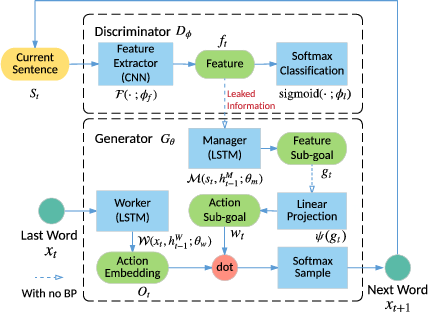
\includegraphics[width=.7\textwidth]{leakgan.png}
  \caption{Architettura di una LeakGAN \cite{LeakGAN}}
  \label{fig:leakgan}
\end{figure}
Va subito fatto notare come la seconda modifica renda il generatore un generatore gerarchico, quindi composto da sottomoduli con specifici compiti.
È altrettanto importante sottolineare che i sotto-compiti che il Manager richiede al Worker sono auto-determinati, infatti i risultati ottenuti dimostrano che il Manger è in grado di richiedere al Worker la generazione di punteggiature e particolari strutture.

La \emph{Linear Projection} presente nello schema effettua una trasformazione lineare $\psi$, con pesi $W_\psi$, su un numero $c$ di goal $g_t$ recenti, così da generare un vettore $w_t$ di dimensione adeguata per l'esecuzione del prodotto con $O_t$.

\noindent
In formule si ha
\begin{align}
  w_t &= \psi \left( \sum_{i=1}^{c} g_{t-1} \right)
  \\
  O_t, h_t &= Worker(x_t, h_{t-1}; \theta)
  \\
  x_{t+1} = G_\theta(\cdot|s_t) &= softmax ( O_t \cdot w_t / \alpha)
\end{align}
in cui $h_t$ è \emph{hidden state} del Worker, mentre $\alpha$ viene usato per bilanciare esplorazione e sfruttamento (\emph{exploration and exploitation}).
In generale avrà un valore alto durante il \emph{training} per favorire l'esplorazione, avrà invece un valore basso durante la generazione di quelle sequenze che poi verranno usate per allenare $D$.

%\todo{spiegare meglio train G? Rescaled $R_t$?}

Un'altra importante modifica riguarda l'\emph{interleaved training}: si alternano allenamento tramite GAN ed allenamento tramite metodo supervisionato (MLE), anziché effettuare soltanto GAN dopo il \emph{pre-train}.
Questo evita il \emph{mode collapse} obbligando $G$ a rimanere aderente alla vera distribuzione degli esempi reali, evitando quindi che si specializzi su casi particolari con cui confondere $D$.
La modifica viene mostrata in modo esplicito a riga 4 del pseudocodice \textbf{Algorithm \ref{alg:LeakGAN}}.
Notare come vengano mostrati esplicitamente i parametri del Worker e del Manager, specificando che vengono aggiornati indipendentemente.
\begin{algorithm}
  \caption{Adversarial Training with Leaked Information}
  \label{alg:LeakGAN}
  \begin{algorithmic}[1]
    \State Initialize $G_{\theta_m, \theta_w}$, $D_\phi$ with random weights $\theta_m$,$\theta_w$, $\phi$
    \State Pre-train $D_\phi$ on real data and generated data
    \State Pre-train $G_{\theta_m, \theta_w}$ using leaked information from $D_\phi$
    \State Perform the two parts of pre-training interleavingly until convergence
    \Repeat
      \For{g-steps}
        \State Generate a sequence $Y_{1:T} = (y_1, \dots, y_T) \sim G_{\theta_m, \theta_w}$
        \For{$t$ in $1:T$}
          \State Store leaked information from $D_\phi$
          \State Get $Q(f_t, g_t)$ by Monte Carlo Search
          \State Get the computed direction $g_t$ from MANAGER
          \State Update WORKER parameters $\theta_w$, $\psi$, softmax
          \State Update MANAGER parameters $\theta_m$
        \EndFor
      \EndFor
      \For{d-steps}
        \State Use current $G_{\theta_m, \theta_w}$ to generate negative examples
        \State Train $D_\phi$ for $k$ epochs on generated examples and real data
      \EndFor
    \Until{LeakGAN converges}
  \end{algorithmic}
\end{algorithm}

I risultati riportati in \cite{LeakGAN} mostrano come le LeakGAN siano in grado di superare le già buone prestazioni delle SeqGAN su sequenze di 20 token e come le superino notevolmente con sequenze lunghe 40 token.
Interessante anche il grafico ottenuto tramite PCA che permette di ottenere una visualizzazione della capacità delle LeakGAN di raggiungere lo spazio delle feature dei dati reali.


In \autoref{tab:esempi} vengono esposti quattro esempi generati da LeakGAN e SeqGAN allenate con le didascalie del dataset COCO.
\begin{table}[ht]
\centering
\begin{tabular}{|l|} 
\hline
LeakGAN  \\
\hline
(1) A man sitting in front of a microphone with his dog sitting oh his shoulder. \\
(2) A young man is holding a bottle of wine in his hand.  \\
\hline
SeqGAN \\
\hline
(1) A couple of kids in a bathroom that is in a bathroom. \\
(2) A bathroom with tiled walls ad shower on it. \\
\hline
\end{tabular}
\caption{Esempi generati da modelli alleanti con \emph{COCO Image Captions}}
\label{tab:esempi}
\end{table}

